\documentclass{article}
\usepackage{amsmath, amssymb,amsfonts,mdframed, tikz,qtree}
\usepackage[ruled,linesnumbered]{algorithm2e}
\usetikzlibrary{shapes,arrows,calc,positioning,backgrounds}
\title{Algorithms \& Complexity: Lecture 14: Coping with $\mathbf{NP}$-hardness II}

\newcommand{\NP}{\mathbf{NP}}
\renewcommand{\P}{\mathbf{P}}

\author{Sam Barrett}

\newmdtheoremenv{lemma}{Lemma}
\newmdtheoremenv{definition}{Definition}
\newmdtheoremenv{theorem}{Theorem}
\newmdtheoremenv{problem}{Problem}
\newmdtheoremenv{example}{Example}

\begin{document}
\maketitle

We have previously seen that $\texttt{IndependentSet} \leq_{P} \texttt{VertexCover}  $ as if $S$ is an independent set, $V\backslash S$ is a vertex cover. I.e. to convert an independent set to a vertex cover, take its compliment and vice vira.

We can therefore say that the time complexity of \texttt{IndependentSet} and \texttt{VertexCover} is the \textbf{same} . Any $f(n)$ time algorithm for one problem also works for the other.

We know that \texttt{VertexCover} is a $\NP$-hard problem but what if we are not concerned with finding the \textbf{minimum} sized vertex cover and instead a cover of some arbitrary size $25$?

\section{Fixed-parameter tractable (FPT) algorithms}

We can define the parameterised vertex cover problem to be the same as the standard vertex cover problem but instead of attempting to find the minimum sized cover we attempt to find a vertex cover of size $\leq k$

We say the paramterised vertex cover problem is fixed-parameter tractable if it can be sovled in $f(k) \cdot n^{O(1)}$ time.

\begin{problem}(The $k$-VC problem)
  Given an undirected graph $G=(V,E)$ on $n$ vertices and a parameter $k$, is there a set $X\subseteq V$ of size $\leq k$ s.t. each edge of $G$ has at least one endpoint in $X$?
\end{problem}

The standard \texttt{VertexCover} problem can then be solved using a series of $O(n)$ calls to the $k$-VC  problem.

If we assume $\P \neq \NP$, we cannot then expect to find an algorithm for $k$-VC which runs in time polynomial in \textbf{both} $k$ and $n$.

We can construct an algorithm for $k$-VC which uses bounded-depth search trees.

This algorithm is best visualised as:

\begin{figure}[ht]
  \centering
  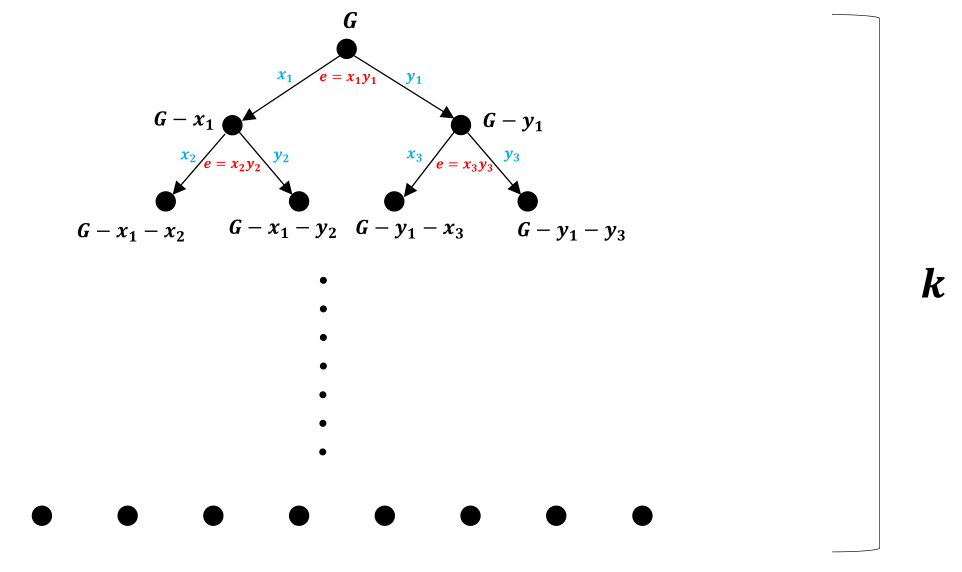
\includegraphics[scale=0.7]{figures/l14-1.png}
  \caption{\label{fig:kvc}FPT $k$-VC algorithm }
\end{figure}

If at least one of the leaf nodes at the bottom of the graph has no edges remaining then there exists a vertex cover of size $\leq k$, otherwise one does not exist.

This algorithm can be seen to have a running time in $2^{k}\cdot n^{O(1)}$. As there are $2^{k}$ leaf nodes for a tree of height $k$ and we must spend $n^{O(1)}$ time at each node to determine if any edges remain.
\end{document}
